\documentclass[11pt]{article}
\usepackage[a4paper,margin=1in]{geometry}
\usepackage{graphicx}
\usepackage{booktabs}
\usepackage{float}
\usepackage{hyperref}
\usepackage{amsmath}
\usepackage{array}
\usepackage{caption}
\usepackage{fancyhdr}
\usepackage{xcolor}
\definecolor{UFBlue}{HTML}{0021A5}
\definecolor{UFOrange}{HTML}{FA4616}
\definecolor{DarkGray}{HTML}{333333}
\hypersetup{colorlinks=true,linkcolor=UFBlue,urlcolor=UFBlue,citecolor=UFBlue}
\setlength{\headheight}{14pt}
\pagestyle{fancy}
\fancyhf{}
\fancyhead[L]{\small\textcolor{UFBlue}{COP5615 --- Distributed Operating Systems Principles}}
\fancyhead[R]{\small\textcolor{DarkGray}{Project 2: Gossip Simulator}}
\fancyfoot[C]{\small\thepage}
\renewcommand{\headrulewidth}{0.5pt}
\setlength{\parindent}{0pt}
\setlength{\parskip}{5pt}
\begin{document}
\hypersetup{pageanchor=false}
% Cover page styled after the supplied UF assignment report.
\begin{titlepage}
\thispagestyle{empty}
\par
\begin{center}
\vspace*{0.35in}

\includegraphics[width=2.65in]{uf_horizontal_logo_cropped.png}
\vspace{0.65in}\\
{\Large\bfseries\textcolor{UFBlue}{%
COP5615 --- DISTRIBUTED OPERATING SYSTEMS PRINCIPLES%
}\par}

\vspace{0.45in}

{\LARGE\bfseries Project 2\par}

\vspace{0.15in}

{\Huge\bfseries\textcolor{UFBlue}{Gossip Simulator}\par}

\vspace{0.25in}

{\color{UFOrange}\rule{4.6in}{1.5pt}}

\vspace{0.35in}
{\large
\begin{tabular}{r l}
\textbf{Student:} & Pradhyuman Singh Shekhawat\\
\textbf{UFID:} & 55742970\\
\textbf{Email:} & pr.shekhawat@ufl.edu\\
\textbf{Term:} & Fall 2026\\
\textbf{Language:} & Erlang\\
\textbf{Algorithms:} & Gossip and Push-Sum
\end{tabular}
}
\vfill
{\small University of Florida\\[2pt]October 2026}
\end{center}
\end{titlepage}
% Preliminary pages use Roman numerals.
\pagenumbering{roman}
\tableofcontents
\clearpage
% Main report uses Arabic numerals.
\clearpage
\pagenumbering{arabic}
\hypersetup{pageanchor=true}
\begin{abstract}
This project implements asynchronous Gossip and Push-Sum simulations
using Erlang actors. Four network topologies are supported: full,
line, two-dimensional grid, and imperfect two-dimensional grid.
A centralized statistics actor collects convergence information and
records elapsed time. Baseline experiments evaluate both algorithms
across network sizes from 4 to 49 nodes. An additional 360-trial
experiment investigates how changing the local Gossip reception
threshold affects convergence. In the baseline experiments, all 72
Push-Sum trials succeeded, whereas 39 of 72 Gossip trials succeeded.
The threshold experiment demonstrates that increasing the local
reception threshold substantially improves observed Gossip success,
particularly for larger and less-connected networks.
\end{abstract}
\par
\section{Introduction}
The objective is to simulate distributed information propagation
using independent Erlang actors communicating through asynchronous
messages. Each actor represents a node in a network and interacts
with its neighbors according to the selected algorithm.
The simulator accepts a node count, topology, and algorithm through
the command-line interface:
\par
\begin{verbatim}
project2 numNodes topology algorithm
\end{verbatim}
Supported topologies are \texttt{full}, \texttt{line}, \texttt{2D},
and \texttt{imp2D}. Supported algorithms are \texttt{gossip} and
\texttt{push-sum}. The experiments use network sizes
\(N \in \{4,9,16,25,36,49\}\). The grid-based topologies use
perfect-square node counts.
\par
\section{Implementation}
\par
\subsection{Actor architecture}
Each simulated node runs as an Erlang process. Actors communicate
using messages rather than shared mutable state. The implementation
separates actor behavior, topology construction, coordination, and
statistics collection.
The coordinator builds the topology, starts the actors, waits for
their registration, configures their neighbors, initiates the selected
algorithm, and waits for the convergence result. A centralized
statistics actor collects actor registrations, algorithm updates,
completion notifications, and convergence information.
Elapsed time is measured with Erlang's monotonic clock. The recorded
duration is the elapsed time between algorithm initiation and the
detected convergence event, expressed in microseconds.
\par
\subsection{Gossip}
Gossip begins when the coordinator sends a rumor to one actor. An
actor that receives the rumor increments its local reception count.
While it remains active, it randomly selects a neighbor and forwards
the rumor. Once its local reception count reaches the configured
threshold, the actor reports completion and stops forwarding the rumor.
The baseline experiments use the default threshold of 10 receptions.
The additional threshold experiment evaluates thresholds of
10, 20, 50, 100, and 500.
The threshold is a \emph{*local reception count per actor*}; it is not
a global number of communication rounds. Because actors operate
asynchronously and select neighbors randomly, a larger threshold
can allow information to continue propagating for longer before
individual actors stop forwarding it.
\par
\subsection{Push-Sum}
Each actor begins with its node identifier as its \(s\) value and
\(w=1\). The actor's current estimate is the ratio \(s/w\). During
communication, an actor divides its current \(s\) and \(w\) values
and sends half to a selected neighbor, retaining the other half.
The implementation uses an epsilon of \(10^{-10}\) and requires
three consecutive stable rounds, as defined by the implementation,
before an actor reports that its estimate has converged. The
coordinator and statistics actor collect the resulting completion
information.
\par
\subsection{Network topologies}
\par
\begin{itemize}
\item \textbf{Full:} each node is connected to all other nodes.
\item \textbf{Line:} nodes are arranged in a linear chain.
\item \textbf{2D grid:} nodes are arranged in a square grid,
with neighbor relationships determined by grid adjacency.
\item \textbf{Imperfect 2D grid:} a two-dimensional grid is
augmented with an additional random neighbor connection.
\end{itemize}
\par
\section{Experimental Methodology}
The baseline dataset contains 144 trials: two algorithms, four
topologies, six network sizes, and three trials per configuration.
The Gossip threshold dataset contains 360 trials: four topologies,
six network sizes, five thresholds, and three trials per
configuration.
A trial is counted as successful when the experiment harness receives
a successful convergence result. Trials without a successful result
are counted as failures. The coordinator uses a 30-second
convergence wait in the current implementation. Therefore, a failed
trial means convergence was not detected successfully within the
experiment's execution conditions; it does not establish that
convergence is mathematically impossible.
For successful trials, the analysis script computes the mean
convergence time and, when at least two successful observations are
available, the sample standard deviation. Failed trials are included
in the success-rate denominator but excluded from convergence-time
averages.
The experiments use only three trials per configuration. The results
should therefore be interpreted as observations of this simulator
under the tested conditions, rather than precise estimates of
long-run success probabilities.
\par
\section{Baseline Results}
\par
\subsection{Overall outcomes}
Table~\ref{tab:baseline} summarizes the baseline success rates by
algorithm and topology. Each entry represents 18 trials:
six network sizes with three trials per size.
\par
\begin{table}[H]
\centering
\caption{Baseline convergence outcomes by algorithm and topology.}
\label{tab:baseline}
\begin{tabular}{llrrr}
\toprule
Algorithm & Topology & Successful & Failed & Success rate \\
\midrule
Gossip & Full & 16 & 2 & 88.9\% \\
Gossip & Line & 7 & 11 & 38.9\% \\
Gossip & 2D & 7 & 11 & 38.9\% \\
Gossip & Imperfect 2D & 9 & 9 & 50.0\% \\
\midrule
Push-Sum & Full & 18 & 0 & 100.0\% \\
Push-Sum & Line & 18 & 0 & 100.0\% \\
Push-Sum & 2D & 18 & 0 & 100.0\% \\
Push-Sum & Imperfect 2D & 18 & 0 & 100.0\% \\
\bottomrule
\end{tabular}
\end{table}
Push-Sum succeeded in all 72 baseline trials, including every
49-node configuration. Gossip was more sensitive to topology and
network size. The full topology had the highest Gossip success rate,
while the line and 2D topologies had the lowest rates in this
baseline dataset.
\par
\subsection{Convergence time}
Figures~\ref{fig:gossip-time} and~\ref{fig:pushsum-time} show the
mean convergence times of successful baseline trials as network size increases. These means
exclude failed trials, so a plotted point does not represent the
expected time to completion across all attempts.
\par
\begin{figure}[H]
\centering
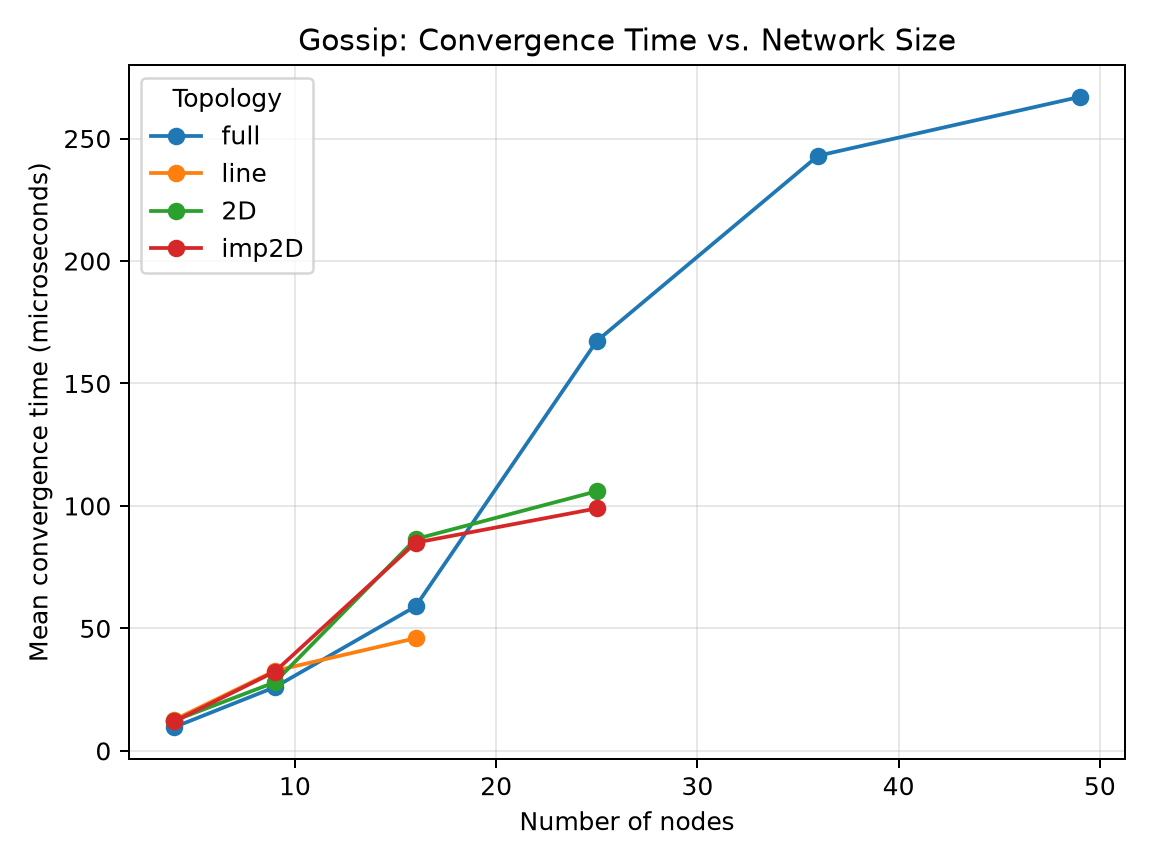
\includegraphics[width=0.88\textwidth]{gossip_convergence.png}
\caption{Mean Gossip convergence time for successful baseline trials.}
\label{fig:gossip-time}
\end{figure}
\par
\begin{figure}[H]
\centering
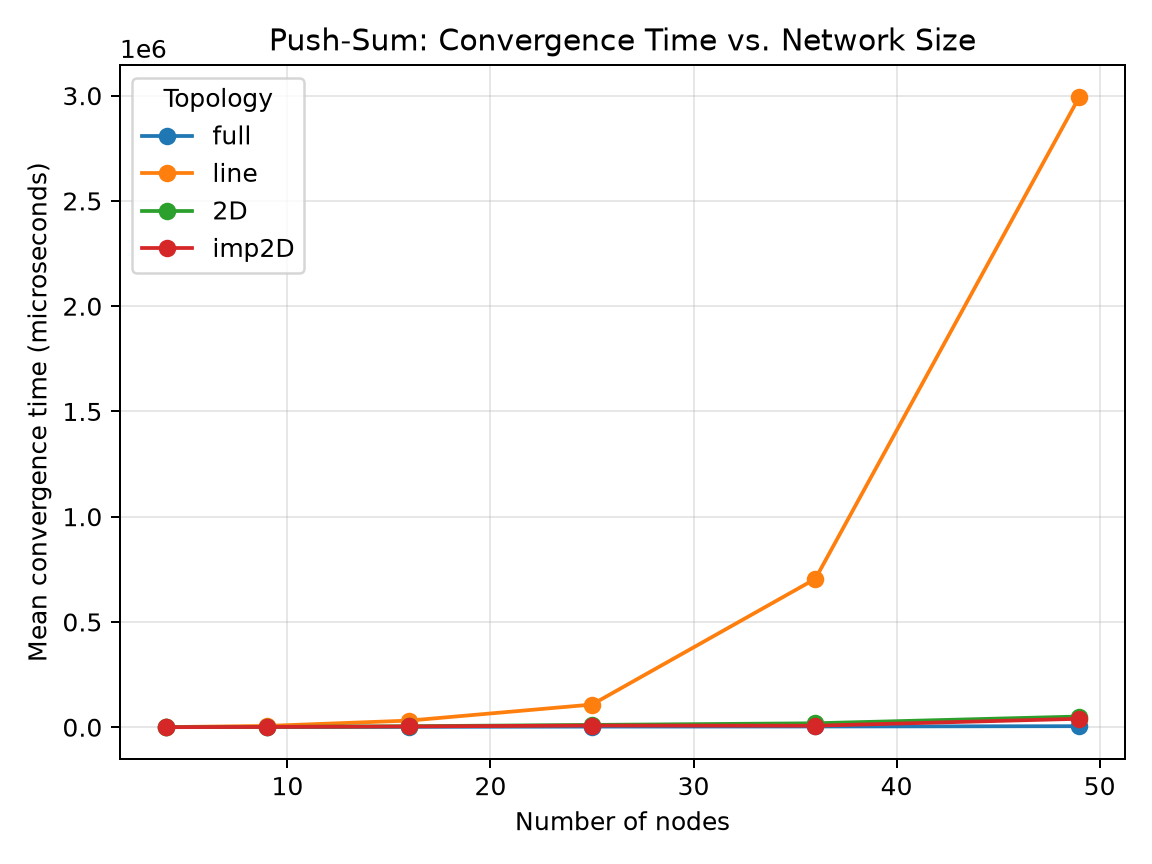
\includegraphics[width=0.88\textwidth]{push-sum_convergence.png}
\caption{Mean Push-Sum convergence time for successful baseline trials.}
\label{fig:pushsum-time}
\end{figure}
Push-Sum's measured convergence time increased substantially with
network size in the line topology. At 49 nodes, the mean successful
line-topology time was approximately 2.99 seconds
(\(2{,}994{,}108\) microseconds). For comparison, the corresponding
full-topology mean was approximately 4.90 milliseconds
(\(4{,}901\) microseconds). This illustrates the impact that network
structure can have on propagation and convergence time in these runs.
For Gossip, the baseline threshold of 10 receptions did not produce
successful convergence in every configuration. In particular, none
of the three baseline trials succeeded for line networks of 25, 36,
or 49 nodes. Mean times for configurations with no successful trials
are omitted rather than interpreted as zero.
\par
\subsection{Largest network with an observed successful trial}
The baseline experiments observed at least one successful Gossip
trial at the following largest tested network sizes:
\par
\begin{center}
\begin{tabular}{lr}
\toprule
Topology & Largest observed successful size \\
\midrule
Full & 49 nodes \\
Line & 16 nodes \\
2D & 25 nodes \\
Imperfect 2D & 25 nodes \\
\bottomrule
\end{tabular}
\end{center}
These sizes describe the baseline threshold of 10 and the tested
network sizes only. They are not maximum capacities of the
implementation. The threshold experiment subsequently observed
successful 49-node Gossip runs on every topology at higher
thresholds.
\par
\section{Gossip Threshold Experiment}
\par
\subsection{Overall success rate}
The additional experiment changes the local reception threshold
while keeping the topology, network sizes, and number of trials
within the same experimental design. Table~\ref{tab:threshold}
shows the aggregate outcomes across all topologies and network sizes.
\par
\begin{table}[H]
\centering
\caption{Gossip outcomes by local reception threshold.}
\label{tab:threshold}
\begin{tabular}{rrrr}
\toprule
Threshold & Successful & Failed & Success rate \\
\midrule
10  & 34 & 38 & 47.2\% \\
20  & 56 & 16 & 77.8\% \\
50  & 64 & 8  & 88.9\% \\
100 & 69 & 3  & 95.8\% \\
500 & 71 & 1  & 98.6\% \\
\bottomrule
\end{tabular}
\end{table}
The observed aggregate success rate increased as the threshold
increased. At threshold 10, fewer than half of the trials succeeded.
At threshold 500, 71 of 72 trials succeeded. This pattern is
consistent with the mechanism of the implementation: actors that
reach their local threshold stop forwarding, and a low threshold can
allow forwarding to stop before all actors have received the rumor.
\par
\begin{figure}[H]
\centering
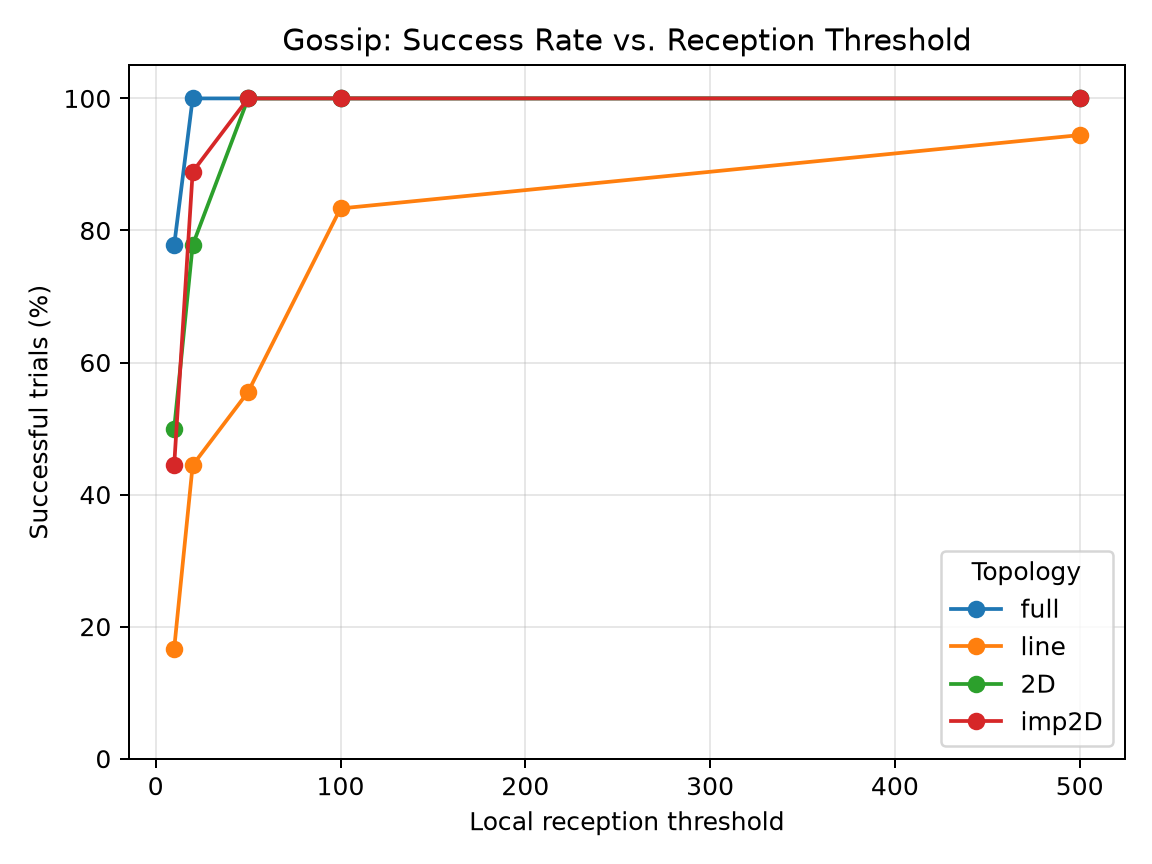
\includegraphics[width=0.88\textwidth]{gossip_threshold_success_rate.png}
\caption{Gossip success rate versus local reception threshold.}
\label{fig:threshold-success}
\end{figure}
\par
\subsection{Topology effects}
Across all five thresholds and six network sizes, each topology
contributes 90 trials. Table~\ref{tab:topology-threshold} summarizes
their outcomes.
\par
\begin{table}[H]
\centering
\caption{Gossip threshold experiment outcomes by topology.}
\label{tab:topology-threshold}
\begin{tabular}{lrrr}
\toprule
Topology & Successful & Failed & Success rate \\
\midrule
Full & 86 & 4 & 95.6\% \\
Line & 53 & 37 & 58.9\% \\
2D & 77 & 13 & 85.6\% \\
Imperfect 2D & 78 & 12 & 86.7\% \\
\bottomrule
\end{tabular}
\end{table}
The line topology remained the most difficult overall. Its limited
neighbor connectivity means that information must travel along the
chain, and randomized forwarding can delay propagation or leave
parts of the network unreached before actors stop forwarding.
The full topology provides many more possible communication paths,
which is consistent with its higher observed success rate.
The imperfect 2D topology performed slightly better than the
regular 2D topology in aggregate in this dataset. The additional
random connection may provide shortcuts, although the small number
of trials does not establish that this difference will always occur.
\par
\subsection{Large line network: follow-up observations}
Two additional runs were recorded separately from the 360-trial
dataset. For a 49-node line at threshold 100, the run timed out;
partial statistics showed rumor-reception reports from only 15 of
the 49 actors. At threshold 500, a subsequent run succeeded, with
all 49 actors represented in the statistics report and a measured
convergence time of 3,686 microseconds.
These two observations are illustrative, not a controlled
comparison. Gossip is randomized, so one successful run and one
failed run cannot by themselves establish a reliable success
probability or typical convergence time. They are consistent with
the larger threshold experiment, in which the 49-node line had no
successes at thresholds 10, 20, or 50, one success at 100, and
three successes at 500.
\par
\begin{figure}[H]
\centering
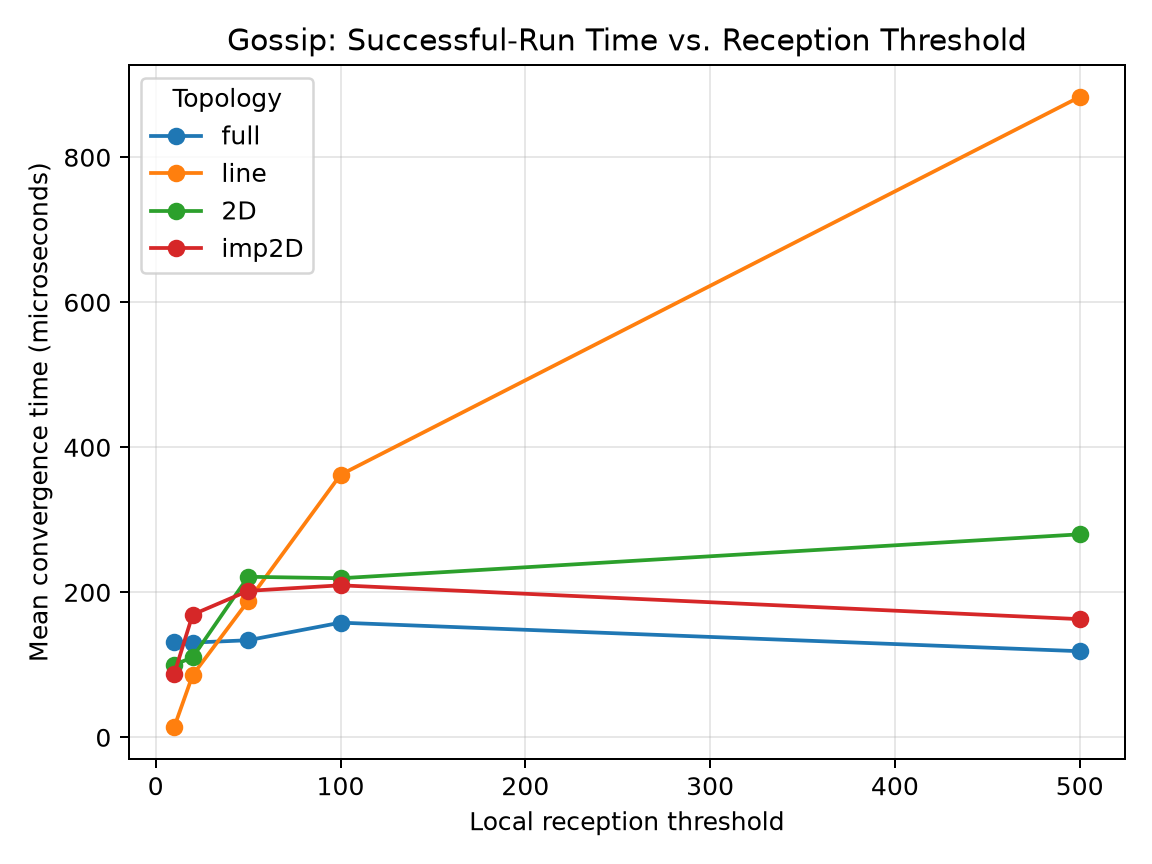
\includegraphics[width=0.88\textwidth]{gossip_threshold_convergence.png}
\caption{Mean convergence time among successful Gossip trials at
each threshold.}
\label{fig:threshold-time}
\end{figure}
The timing graph must be interpreted alongside the success-rate
graph. A threshold can have a low mean time among successful runs
while still failing frequently, because unsuccessful runs are not
included in the mean. Success rate and convergence time therefore
provide complementary measures of the experiment.
\par
\section{Discussion and Limitations}
The experiments support several conclusions about the implemented
simulator:
\par
\begin{enumerate}
\item \textbf{Topology matters.} Gossip was more reliable on the
full topology than on the line topology in both the baseline and
threshold experiments.
\item \textbf{The local stopping threshold matters.} Increasing
the Gossip reception threshold was associated with higher
aggregate success rates in the tested runs.
\item \textbf{Push-Sum was reliable in the baseline runs.}
All 72 tested trials succeeded, but this does not guarantee
success for all larger networks or other execution conditions.
\item \textbf{Reliability and speed must be considered together.}
Successful-run mean time excludes failures and should not be
interpreted independently of the success rate.
\end{enumerate}
There are important limitations. Only three trials were run for each
configuration, and randomized execution can produce substantial
variation. The tested network sizes stop at 49 nodes. The reported
results are also specific to the implementation's stopping criteria
and timeout. The threshold experiment varies a local reception count,
not a synchronized global round count. Finally, the two follow-up
runs are supplementary observations and are not included in the
aggregate trial counts.
Future work could increase the number of trials, test larger networks,
record explicit failure reasons, and compare additional stopping
criteria. Repeating the experiments with fixed, recorded random seeds
would also improve reproducibility.
\par
\section{Conclusion}
The Erlang simulator implements asynchronous Gossip and Push-Sum
over four network topologies and records convergence statistics.
In the baseline experiments, Push-Sum succeeded in all 72 trials,
while Gossip succeeded in 39 of 72. Gossip's success was sensitive
to topology, with the line network presenting the greatest
difficulty.
The 360-trial threshold experiment found that aggregate Gossip
success increased from 47.2\% at threshold 10 to 98.6\% at threshold
500. The results demonstrate why the local stopping threshold must
be considered when interpreting Gossip convergence. These findings
are limited to the tested sizes, three repetitions per configuration,
and the current implementation and timeout settings.
\end{document}